% !TEX encoding = UTF-8
% !TEX TS-program = pdflatex
% !TEX root = ../tesi.tex
% !TEX spellcheck = it-IT

%**************************************************************
\chapter{Progettazione e realizzazione}
\label{cap:progettazione-realizzazione}
%**************************************************************

%\intro{}\\

%**************************************************************
%**************************************************************
%**************************************************************

\section{Strumenti utilizzati}
  \subsection{Hardware e sistema operativo}	  
    Il lavoro sul progetto non ha richiesto particolari risorse \textit{hardware}, ed ho potuto	
    utilizzare il mio portatile con Linux Ubuntu 14.04 (\textit{Trusty Tahr}) per lo sviluppo, nonostante questo
    non fosse un requisito obbligatorio per lavorare sul progetto; infatti \textbf{Speect} è un sistema portabile
    su tutte le maggiori piattaforme.
  \subsection{Linguaggi di programmazione e librerie esterne}
   L'\textit{engine} di \textbf{Speect} è sviluppato interamente in linguaggio \textit{C}, e permette di sviluppare i \textit{plug-in}
   in \textit{C} o in \textit{Python}. Durante questo \textit{stage} è stato utilizzato il linguaggio \textit{C}. \\
   Oltre al \textit{C} sono stati utilizzati i linguaggi \textit{bash} per l'attività di \textit{testing} e \hyperref[glo:xsl]{\emph{XSL}\glsfirstoccur}
   per l'elaborazione
   di alcuni \textit{file} \textit{XML} generati da alcuni processi di \textbf{Speect}. \\ 
   L'unica libreria esterna utilizzata nel progetto è \href{http://xmlsoft.org/}{LibXML2}, utilizzata nel \textit{plug-in} 
   \texttt{maryxml} per scrivere parte del contenuto dell' \textit{HRG} nel formato di \textit{output} definito 
   da \textbf{MaryTTS}, \href{http://mary.dfki.de/documentation/maryxml/}{MaryXML}. È stata scelta per i seguenti motivi:
   \begin{itemize}
      \item è scritta in \textit{C};
      \item è molto utilizzata;
      \item è rilasciata con \textit{licenza MIT}, la stessa con cui è rilasciato \textbf{Speect}.
   \end{itemize}

  \subsection{Strumenti per il \textit{building}} 
    \begin{itemize}
	\item \textbf{CMake}: è un generatore di sistemi di compilazione \textit{cross-platform}. Un progetto che utilizza questo \textit{tool} deve specificare
	      		      il processo di \textit{build} tramite dei \textit{file} indipendenti dalla piattaforma chiamati \texttt{CMakeLists.txt}, i quali 
			      devono far parte di ciascuna cartella dell'albero delle \textit{directory} del progetto;

        \item \textbf{Automake}: è un \textit{tool} per la generazione automatica di \textit{file} chiamati \texttt{Makefile.in} a partire
	      			 da \textit{file} chiamati \texttt{Makefile.am}. Questi contengono delle liste di definizioni di variabili
				 per il programma \textit{make} e di regole. I \textit{file} \texttt{Makefile.am} sono compatibili con gli 
				 \textit{standard} \textbf{GNU Makefile};
	\item \textbf{Autoconf}: è un \textit{tool} creato da \textit{GNU} che permette la creazione di pacchetti generando uno \textit{script bash}
                                 (chiamato \texttt{configure}) a partire da un \textit{file} chiamato \texttt{configure.ac},
	      			 il quale a sua volta è in grado di produrre un \textit{file} \texttt{Makefile}.
    \end{itemize}

   \subsection{Versionamento}
      \begin{figure}[!h] 
        \centering 
        
\includegraphics[width=0.5\columnwidth]{git-logo} 
        \caption{Logo di \textit{git}}
      \end{figure} 

      Per il controllo di versione l'azienda utilizza il \textit{software} \textit{git}, abbinato ai seguenti servizi per l'\textit{hosting}: 
      \begin{enumerate}
	\item \textbf{GitHub}: utilizzato per l'\textit{hosting} di un \textit{repository} pubblico contenente il codice 
	      		       di \textbf{Speect};
	\item \textbf{GitLab}: utilizzato per l'\textit{hosting} di un \textit{repository} privato contenente alcuni 
	      		       \textit{tool} interni all'azienda  per il \textit{building} ed il \textit{testing} di \textbf{Speect}.

	\paragraph{Workflow per git}
        Per quanto riguarda il \textit{workflow} nell'utilizzo di \textit{git} e \textit{GitHub}, la politica aziendale impone
	di creare un \textit{fork} del \textit{repository} dell'azienda e di contribuire al progetto da tale \textit{fork}.
	Pertanto ho sempre eseguito i \textit{commit} ed i \textit{push} avendo come riferimento il mio \textit{fork} personale;
	il codice da me prodotto è stato sempre integrato dal \textit{tutor} aziendale nel \textit{repository} dell'azienda tramite
 	\textit{rebasing}. \\ Le norme da seguire nella partecipazione al progetto sono state dunque le seguenti:
        \begin{itemize}
           \item un \textit{commit} deve riguardare un singolo \textit{file}, e le modifiche contenute in esso
              devono avere un unico obiettivo;
           \item una volta terminato un \textit{task}, si effettua un \textit{push} sul \textit{fork} personale;
           \item si effettua una richiesta di integrazione all'integratore (nel nostro caso al \textit{tutor} aziendale), il quale
                 può:
                    \begin{itemize}
                      \item accettarla ed integrare i \textit{commit} nel \textit{fork} principale del progetto;
                      \item rifiutarla e richiedere modifiche ai \textit{commit}.
                    \end{itemize}
        \end{itemize}
        
      \end{enumerate}

%*************************************

\section{Il \textit{plug-in} maryxml}
Come introduzione al sistema e ai \textit{plug-in} mi è stato chiesto di effettuare alcune modifiche
al \textit{plug-in} \texttt{maryxml}, il quale è stato creato dai due tirocinanti precedenti con lo scopo
di confrontare l'\textit{output} generato da \textbf{Speect} con l'\textit{output} di \textbf{MaryTTS}.
   \subsection{Il formato \textit{MaryXML}}
      \textbf{MaryTTS} utilizza il metalinguaggio \textit{XML} per la trattazione dei dai interni. \\
             Il linguaggio definito tramite \textit{XML Schema} all'interno di \textbf{MaryTTS} prende il nome
             di \textit{MaryXML}. L'utilizzo di \textit{XML} comporta i seguenti:
                  \begin{itemize}
                    \item vantaggi:
                         \begin{itemize}
                            \item rigidità fornita dal metalinguaggio;
                            \item facilità nel manipolare i dati;
                            \item possibilità di avere \textit{file} sempre validi.
                         \end{itemize}
                    \item svantaggi:
                         \begin{itemize}
                           \item impossibilità da parte degli utenti di modificare gli schemi;
                           \item le modifiche sono possibili soltanto negli schemi locali.
                         \end{itemize}
                  \end{itemize}
                  \textbf{MaryTTS} utilizza il linguaggio \textit{MaryXML} per tutti i \textit{file} interni,
                  compresi quelli riguardanti la voce. In \textbf{MaryTTS}, ogni lista di fonemi, dizionario o rappresentazione
                  dei \textit{token} deve seguire lo schema definito per \textit{MaryXML}. \\ Data la rigidità dello schema, l'aggiunta
                  di nuovi elementi o attributi è possibile solamente dopo le modifiche degli \textit{schema} locali 
                  e delle classi per la lettura dei nuovi elementi/attributi. \\
                  In \hyperref[app:appc]{Appendice C} viene riportato un esempio di \textit{file} \textit{MaryXML}.
                  \paragraph{Nota su Speect} A differenza di \textbf{MaryTTS}, \textbf{Speect} per trattare
                  i \textit{file} interni utilizza il linguaggio \textit{JSON}, il quale permette di fornire
                  maggiore libertà all'utente definendo un numero ristretto di regole.
         \subsection{Scopo del \textit{plug-in}}
             Il \textit{plug-in} ha lo scopo di scrivere su \textit{file} i \textit{token} generati e normalizzati
             di \textbf{Speect}. \\
             Sostanzialmente questa componente richiede all'\textit{HRG} i \textit{token} da stampare e li scrive su \textit{file} 
             in formato \textit{MaryXML}. \\
             Prima del mio \textit{stage} non venivano stampati i dati riguardanti le sillabe, dunque il mio contributo
             a questo \textit{plug-in} consiste nell'aver ricavato questi dati dall'\textit{HRG} e nell'averli stampati
             in formato \textit{MaryXML}. \\
             Di seguito vengono riportati due \textit{output} provenienti dall'elaborazione dell'\textit{input} 'Ciao' 
             (rispettivamente prima e dopo il mio contributo):
             \begin{itemize}
               \item \textit{senza} i dati relativi alle sillabe: \\
                 \begin{lstlisting}[language=XML] 
                   <t pos="SP" ph="tS a - o">ciao</t> 
                 \end{lstlisting}
               \item \textit{con} i dati relativi alle sillabe: \\
                 \begin{lstlisting}[language=XML] 
                   <t pos="SP" ph="tS a - o">ciao<syllable><ph p="tS"/><ph p="a"/></syllable><syllable><ph p="o"/></syllable></t>
                 \end{lstlisting}
             \end{itemize}
%*************************************

\section{Sviluppo del sillabificatore}
\label{sec:progettazione}
All'inizio del periodo di \textit{stage} \textbf{Speect} non includeva tra i suoi \textit{utterance processor} un sillabificatore
per la lingua italiana, perciò negli esperimenti dell'azienda gli \textit{input} in lingua italiana venivano sillabificati secondo le regole
della lingua inglese, riducendo così la qualità dell'\textit{output} prodotto.
%Marina Nespor, "Le strutture del linguaggio - Fonologia"
%Pietro Maturi, "I suoni delle lingue, i suoni dell'italiano"
%T.A. Hall, "English syllabification as the interaction of markedness constraints", Studia Linguistica, vol. 60, 2006, pp. 1-33 --> link
%https://www.researchgate.net/publication/227729497_English_syllabification_as_the_interaction_of_markedness_constraints
\subsection{I due approcci alla sillabificazione}
Tradizionalmente il problema della sillabificazione è affrontato definendo delle sequenze di fonemi (dette \textit{cluster}) valide per 
una determinata lingua, e definendo regole di sillabificazione opportune sulla loro base. \\ Per l'implementazione del sillabificatore
il \textit{tutor} aziendale ha proposto un algoritmo basato sulla variazione della sonorità dei fonemi che riduce la necessità di 
codificare esplicitamente i \textit{cluster} di fonemi di una lingua.
      \subsubsection{Sillabificazione per \textit{cluster}}
           È il metodo utilizzato dal \textit{plug-in} già esistente in \textbf{Speect} per l'inglese, teorizzato
           nell'articolo 
           \href{http://www.zas.gwz-berlin.de/fileadmin/material/ZASPiL_Volltexte/zp37/zaspil37-hall.pdf}
           {\textit{English syllabification as the interaction of markedness constraints}} di T.A. Hall. \\
           Quest'ultimo propone delle azioni predefinite in base ai \textit{cluster} di fonemi incontrati nella stringa di \textit{input} durante il suo \textit{parsing}. \\
           Nella trattazione seguente verranno utilizzati i seguenti simboli:
           \begin{itemize}
             \item \textbf{C}: rappresenta una consonante;
             \item \textbf{G}: rappresenta una semivocale;
             \item \textbf{V}: rappresenta un picco di sonorità all'interno di una sillaba, che può consistere in:
                               \begin{itemize}
                                 \item una \textit{vocale breve};
                                 \item una \textit{vocale lunga};
                                 \item un \textit{dittongo};
                                 \item una \textit{sonorante sillabica}.
                               \end{itemize}
           \end{itemize}
           Nella seguente tabella vengono riportati alcuni esempi di regole tratti dall'articolo citato (il simbolo '.' viene usato come
           separatore tra le sillabe): \newpage
           %BEGIN of table section
           \begin{center}
             \begin{longtable}{ | >{\centering}p{2cm} | >{\centering}p{4cm} | >{\centering}p{1.5cm} | >{\centering}p{2cm} | }
               \hline
               \textbf{Cluster} & \textbf{Possibili sillabificazioni} \tabularnewline \hline
                % example & bla \tabularnewline \hline
                 VCV & V\textbf{.}CV  \tabularnewline \hline
                 VCCV & V\textbf{.}CCV, VC\textbf{.}CV  \tabularnewline \hline
                 VCCCV & VC\textbf{.}CCV, VCC\textbf{.}CV  \tabularnewline \hline
                 VCCCCV & VC\textbf{.}CCCV  \tabularnewline \hline
                 VCGV & VC\textbf{.}GV, V\textbf{.}CGV, VC\textbf{.}GV  \tabularnewline \hline
                 VCCGV & V\textbf{.}CCGV  \tabularnewline \hline
                 VCCCGV & VC\textbf{.}CCGV  \tabularnewline \hline
             \end{longtable}
           \end{center}
           %END of table section
         %  \begin{itemize} 
             \paragraph{Vantaggi} 
               Il presente metodo è abbastanza semplice da implementare, inoltre è ben documentato nell'articolo di T.A. Hall.
             \paragraph{Svantaggi} 
               Gli svantaggi principali della sillabificazione per \textit{cluster} sono la verbosità nella sua implementazione
               e il comportamento non definito in caso di \textit{input} non ben formati secondo le regole della lingua in esame.  
         %  \end{itemize}
      \\
      \subsubsection{Sillabificazione per sonorità} 
      Il metodo si basa su alcuni semplici principi riguardanti la sonorità dei fonemi all'interno di una sillaba, proposti da 
      Pietro Maturi in \href{https://www.mulino.it/isbn/9788815133052}{\textit{I suoni delle lingue, i suoni dell'italiano}}. \\
      Di questo algoritmo esistono due sole implementazioni, una parziale in \textit{Java} di Giulio Paci (il \textit{tutor} aziendale), 
      e quella discussa in questo documento, completa e in \textit{C}.
      Innanzitutto viene stabilita una \textit{scala di sonorità} dei fonemi in base alla loro tipologia, presentata qui in ordine
      di sonorità crescente dal primo all'ultimo elemento della lista:
      \begin{enumerate}
        \item {\hyperref[glo:consoccl]{consonanti \emph{occlusive}\glsfirstoccur}};
        \item {\hyperref[glo:consfric]{consonanti \emph{fricative}\glsfirstoccur}};
        \item {\hyperref[glo:consnasa]{consonanti \emph{nasali}\glsfirstoccur}};
        \item {\hyperref[glo:conslate]{consonanti \emph{laterali}\glsfirstoccur}};
        \item \textit{s sorda}: questo fonema viene trattato singolarmente in questa posizione per evitare
          l'introduzione di ulteriori regole proposte nell'articolo di Maturi.\\  Di fatto questo trattamento per
          la 's sorda' elimina anche la necessità di utilizzare alcuni \textit{cluster} proposti nello stesso articolo;
        \item {\hyperref[glo:consvibr]{consonanti \emph{vibranti}\glsfirstoccur}};
        \item {\hyperref[glo:consappr]{consonanti \emph{approssimanti}\glsfirstoccur}};
        \item vocali.
      \end{enumerate}
      Una parola è dunque costituita dall'alternanza di suoni più o meno \textit{intensi},
      per cui l'algoritmo di sillabificazione per sonorità può
      essere riassunto nel modo seguente: \\ \\
         %   \begin{center}
                \texttt{Data una lista di zero o più consonanti comprese tra due vocali v1 e v2, il punto di inizio della sillaba
                   contenente v2 è situato nel punto in cui la sonorità non decresce spostandosi nel verso che va da v2
                   a v1.} \\ \\
        %    \end{center}
          
      %La seguente immagine dovrebbe rendere più chiaro il funzionamento di questo metodo: 
      % serve un'immagine di una parola con le frecce
      % \begin{figure}[!h] 
      %  \centering 
      %  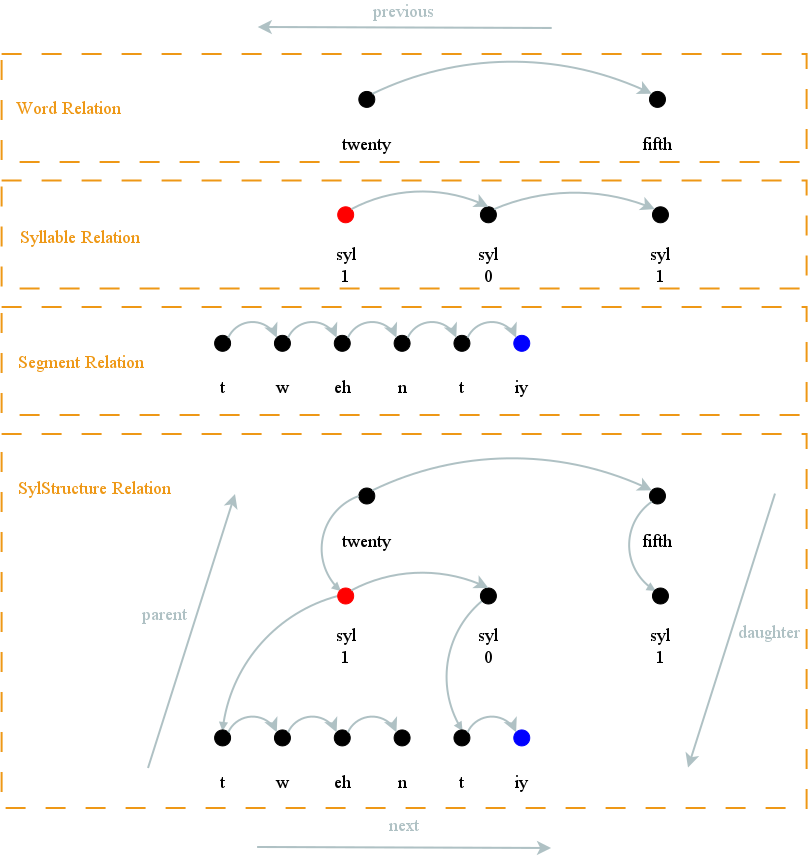
\includegraphics[width=0.9\columnwidth]{hrg} 
      %  \caption{Esempio di \textbf{H}eterogeneous \textbf{R}elation \textbf{G}raph}
      %  \end{figure}
      Questo metodo funziona nella maggior parte dei casi, tuttavia l'attività di \textit{testing} ha permesso 
      di individuare dei casi (gestiti con opportune eccezioni)
      in cui l'algoritmo fornito sopra produce \textit{output} scorretti:
      \begin{itemize}
        \item {\hyperref[glo:consappr]{consonanti \emph{approssimanti}\glsfirstoccur}} adiacenti: 
              i due fonemi devono rientrare nella stessa sillaba;
              \label{exc:apprappr}
        \item {\hyperref[glo:consoccl]{consonante \emph{occlusiva}\glsfirstoccur}} seguita da una 
              {\hyperref[glo:consnasa]{consonante \emph{nasale}\glsfirstoccur}}: i due fonemi devono appartenere a due sillabe diverse;
              \label{exc:occlnasa}
        \item {\hyperref[glo:consoccl]{consonante \emph{occlusiva}\glsfirstoccur}} seguita da un'altra 
              {\hyperref[glo:consoccl]{consonante \emph{occlusiva}\glsfirstoccur}}: i due fonemi devono appartenere a due sillabe diverse;
              \label{exc:occloccl}
        \item {\hyperref[glo:conslate]{consonante \emph{laterale}\glsfirstoccur}} seguita dalla consonante \textit{s}: 
              i due fonemi devono appartenere a due sillabe diverse;
              \label{exc:lates}
        \item {\hyperref[glo:consnasa]{consonante \emph{nasale}\glsfirstoccur}} seguita dalla consonante \textit{s}: 
              i due fonemi devono appartenere a due sillabe diverse.
              \label{exc:nasas} 
      \end{itemize}

           %\begin{itemize}
             \paragraph{Vantaggi}
                     È molto meno verboso rispetto al metodo precedente, fatto che si concretizza in una dimensione del codice molto
                     più ridotta (la riduzione del numero di righe di codice è stata del 65\%). \\ Inoltre permette di gestire 
                     qualsiasi \textit{input}, compresi
                     quelli che non rispettano le regole della lingua in esame.
             \paragraph{Svantaggi}
                    L'implementazione di questo algoritmo richiede maggiore attenzione rispetto alla sillabificazione per \textit{cluster}.
           %\end{itemize}



%**************************************************************

%**************************************************************
\section{Calcolo e raccolta delle \textit{feature}}
I \textit{feature processor} hanno lo scopo di calcolare alcuni attributi propri di varie componenti dell'\textit{input},
tra cui fonemi, sillabe e frasi, attributi che in seguito verranno scritti come campi dati degli \textit{item} del grafo \textit{HRG}. \\
Esempi di \textit{feature} sono i seguenti (di seguito ne vengono riportate soltanto le descrizioni testuali):
\begin{itemize}
  \item livello \textit{phrase}: numero di \textit{phrase} successive a quella corrente nell'\textit{utterance};
  \item livello \textit{phoneme}: {numero di \textit{phoneme} successivi a quello corrente dentro la sillaba}.
\end{itemize}

Le \textit{feature} calcolate dai \textit{feature processor} sono utili in quanto vengono sfruttate dal \textit{vocoder} per
la sintesi dell'\textit{input} fornitogli dal \textit{front-end}. Il \textit{vocoder} di cui fa uso attualmente \textbf{Speect} è 
\href{http://hts-engine.sourceforge.net/}{HTS engine}. \\ 
Tuttavia \href{http://hts-engine.sourceforge.net/}{HTS engine} richiede che le \textit{feature} gli siano passate sotto forma di codici 
alfanumerici, da qui in poi denominati \textit{htslabel}. In generale le \textit{htslabel} sono delle etichette arbitrarie, ma, poiché vengono
utilizzate dal \textit{back-end} come chiavi di ricerca all'interno di un \textit{database} per trovare i parametri necessari alla produzione di audio, 
esse devono avere lo stesso formato di quelle utilizzate durante la fase di creazione dei \textit{database}. Per poter utilizzare i \textit{database} 
di cui si serve \textbf{MaryTTS} è perciò necessario effettuare una mappatura tra i nomi 
delle \textit{feature} in \textbf{Speect} e i codici \textit{hts} corrispondenti definiti da \textbf{MaryTTS} (parte dell’attività di mappatura era 
già stata svolta prima dello \textit{stage}). \\
Sono stati dunque corretti ed ampliati due \textit{plug-in}, \texttt{hts\_label\_data\_collector} e \texttt{hts\_label\_generator\_it}.

\begin{figure}[!h] 
    		\centering 
    		
\includegraphics[width=0.4\columnwidth]{hts_logo} 
   	 	\caption{Logo di \textit{HTS engine}}
\end{figure}


      \subsection{Il \textit{plug-in} hts\_label\_data\_collector}
		Il \textit{plug-in} era già in uno stadio avanzato (se si esclude un \textit{segmentation fault} causato
                da un'istruzione di \textit{return} mancante) prima dello \textit{stage}. \\
		Sostanzialmente esso costituisce un \textit{hub} avente il compito di ricavare i dati dai 
                \textit{feature processor} disponibili
		e di scrivere i nomi e i valori delle \textit{feature} da essi calcolate nei nodi dell'\textit{HRG}. \\
                I nomi delle \textit{feature} sono del tutto arbitrari (infatti sono stati stabiliti da un altro tirocinante),
		ma univoci, in quanto devono poter essere usati come chiavi per la ricerca dei valori corrispondenti. \\
                La tabella 4.2 riporta le relazioni tra alcune \textit{feature} e alcuni \textit{feature processor}, con le descrizioni
                del significato delle \textit{feature}.
                \newpage
                %COMMENTO: serve una tabella con qualche feature e il plugin usato per calcolarla,
		%COMMENTO: negli appunti 20_06.txt ci sono le associazioni
		\begin{center}
        		\bgroup
        		\def\arraystretch{1.8}
        		\begin{longtable}{ | l | p{2cm} | p{4.7cm} | p{2.5cm} |}
        		\hline
        		\textbf{Feature} & \textbf{Descrizione}
        		& \textbf{Feature Processor} \\ \hline
        		\texttt{phrase.syls.num} & numero di sillabe nella \textit{phrase} & \texttt{phrase\_num\_syls} \newline  \\ \hline
        		\texttt{phrase.words.num} & numero di \textit{word} nella \textit{phrase} & \texttt{phrase\_num\_words} \newline  \\ \hline
       			\texttt{phrases.from.utt.end} & numero di \textit{phrase} successive a quella corrente nell'\textit{utterance}  & \texttt{phrase\_pos\_utt\_rev} \newline  \\ \hline
        		\texttt{phrases.from.utt.start} & numero di \textit{phrase} successive a quella corrente nell'\textit{utterance} & \texttt{phrase\_pos\_utt} \newline  \\ \hline
         
        		\texttt{phones.from.syl.end} & numero di \textit{phoneme} successivi a quello corrente dentro la sillaba & \texttt{segment\_pos\_syl\_end} \newline  \\ \hline
        		\texttt{phones.from.syl.start} & numero di \textit{phoneme} precedenti a quello corrente dentro la sillaba & \texttt{segment\_pos\_syl} \newline  \\ \hline
       			\texttt{utterance.phrases.num} & numero di \textit{phrase} nella \textit{utterance} corrente & \texttt{utt\_num\_phrases}  \newline  \\ \hline
        	 	\texttt{syl.phones.num} & numero di \textit{phoneme} nella sillaba corrente & \texttt{syllable\_num\_phones} \newline  \\ \hline                 

       			\texttt{syls.from.phrase.end} & numero di sillabe nella \textit{phrase} corrente & \texttt{syllable\_pos\_phrase\_rev}  \newline  \\ \hline
        		\texttt{syls.from.phrase.start} & numero di sillabe precedenti a quella corrente nella \textit{phrase}  & \texttt{syllable\_pos\_phrase} \newline  \\ \hline
       			\texttt{syls.from.prev.accent} & numero di sillabe successive all'ultima sillaba accentata & \texttt{syllable\_accent\_all\_in} \newline  \\ \hline

        	        \caption{Feature e Feature Processor}
        	        \end{longtable}
        	        \egroup
     	        \end{center}
    	%END of table
     \subsection{Il \textit{plug-in} hts\_label\_generator\_it}
		 Questo \textit{plug-in} si occupa della costruzione dell'\textit{output} per \textit{HTS engine} ricavando i dati
		 necessari  dal \textit{plug-in} precedente. \\ Sostanzialmente esso si occupa di invocare il \textit{plug-in}
		 \texttt{hts\_label\_data\_collector} e di salvare i dati da esso raccolti in una stringa, la quale 
		 in seguito verrà mandata in \textit{output} su \textit{file}.  \\
		 La struttura e le funzionalità di base del presente \textit{plug-in} erano già state sviluppate
		 da un altro tirocinante, tuttavia sono state apportate le seguenti modifiche:
		 \begin{itemize}		
			\item molte \textit{feature} calcolate dal \textit{plug-in} \texttt{hts\_label\_data\_collector}
			      non venivano effettivamente utilizzate e quindi non risultavano nell'\textit{output}
			      finale: si è dunque provveduto a ricavare una parte significativa delle \textit{feature}
			      calcolate. \\ Lo scopo primario di tale attività è stato generare un \textit{output}
			      con il maggior numero possibile di informazioni, fornendo così a \textit{HTS engine} un \textit{input}
			      più completo;
			\item analizzando il codice esistente del presente \textit{plug-in} è stato notato come i nomi
			      delle \textit{feature} (all'interno di \textbf{Speect}) e i codici \textit{hts} corrispondenti
			      fossero presenti come stringhe all'interno del codice. \\ È stato dunque considerato opportuno
			      un certo grado di parametrizzazione, ponendo la mappatura tra nomi in \textbf{Speect} e codici
			      \textit{hts} all'interno del \textit{file} di configurazione \texttt{voice.json}.
		 \end{itemize} 
                 La parametrizzazione del \textit{plug-in} citata sopra ha permesso di spostare il problema dell'aggiunta delle
                 \textit{feature} nella configurazione. \\ Questo fatto assume una grande importanza in quanto ora il \textit{plug-in} 
                 è generico: ciò significa che, a meno di correzioni e di piccoli miglioramenti, non è più necessario modificarlo
                 per estenderne l'\textit{output}; in questo modo l'estensione a nuove lingue e voci diventa più agevole
                 (in precedenza era necessario riscrivere il \textit{plug-in} per ogni impostazione). \\
                 Dunque, grazie a questa nuova impostazione, l'aggiunta di nuove \textit{feature} (se ricavate dal
                 \textit{plug-in} \texttt{hts\_label\_data\_collector})
                 non richiede più alcuna modifica del codice del presente \textit{plug-in}.


      \subsection{Utterance processor 'Prosody'}
                Per replicare le componenti di \textbf{MaryTTS} che calcolano le informazioni di intonazione prosodica è stato necessario 
                introdurre un nuovo \textit{plug-in}, \texttt{rule\_based\_features}, che implementasse un nuovo \textit{utterance processor} 
                chiamato \texttt{Prosody}. \\ Prima del mio \textit{stage} nessuna \textit{feature} era stata calcolata tramite questo metodo
                (per motivi di tempo i due tirocinanti precedenti e il \textit{tutor} aziendale non si sono dedicati a questo lavoro),
                pertanto la realizzazione del presente \textit{plug-in} ha previsto lo studio delle analoghe componenti di \textbf{MaryTTS},
                la progettazione della componente e la sua implementazione. \\
                
                \paragraph{Descrizione del metodo utilizzato}
                Il valore di alcune \textit{feature} può essere ricavato attraverso l'applicazione di semplici \textit{regole},
                le quali sono esprimibili nella seguente forma:
	\\ \\
          \texttt{Dato un nodo del grafo HRG, se esso è caratterizzato da una feature \textit{x} con valore \textit{v}, e questo
		  valore appartiene ad una lista \textit{Lv}, allora si può impostare una feature \textit{y} ad un valore \textit{w}. \\
		  Se la regola precedente fallisce, ne vengono applicate altre a cascata fino ad una regola che ha successo oppure fino
		  all'esaurimento di tutta la sequenza di regole.} \\ 

                L'\textit{engine} \textbf{MaryTTS} calcola alcune \textit{feature} tramite questo metodo,
                ma pone liste di valori e regole insieme all'interno
                di un \textit{file} di configurazione \textit{XML}. \\ Per l'implementazione di questo \textit{plug-in} è stato ritenuto opportuno	
                (almeno in una prima fase) mantenere separati i dati e le azioni corrispondenti alle regole. \\ Pertanto alcune liste di valori
                del \textit{file} \textit{XML} di \textbf{MaryTTS} citato sopra sono state riportate nel \texttt{voice.json}, tra i dati  
                associati all'\textit{utterance processor} \texttt{Prosody}.
                \paragraph{Esempi di regole}
                  \begin{itemize}
                    \item \textbf{regola sulla lista pos\_tonal\_accent}: se il valore della \textit{feature} 
                                                                          \texttt{POS} (che rappresenta il \texttt{part-of-speech tag} 
                                                                          associato all'\textit{item}) del \textit{word item} 
                                                                          è contenuto nella lista chiamata \texttt{pos\_tonal\_accent}
                                                                          (è una lista di valori contenuta nel \textit{file} di configurazione),
                                                                          allora il valore della \textit{feature} \texttt{accent} del \textit{word item}
                                                                          va impostato alla stringa \texttt{tone};
                    \item \textbf{regola sulla lista pos\_no\_accent}:    se il valore della \textit{feature} 
                                                                          \texttt{POS} (che rappresenta il \texttt{part-of-speech tag} 
                                                                          associato all'\textit{item}) del \textit{word item} 
                                                                          è contenuto nella lista chiamata \texttt{pos\_no\_accent}
                                                                          (è una lista di valori contenuta nel \textit{file} di configurazione),
                                                                          allora il valore della \textit{feature} \texttt{accent} del \textit{word item}
                                                                          va impostato alla stringa vuota;
                    \item \textbf{regola di default}:                     in caso di fallimento delle due regole precedenti,
                                                                          allora il valore della \textit{feature} \texttt{accent} del \textit{word item}
                                                                          va impostato alla stringa vuota;
                    \item \textbf{regole sul tipo di frase}:
                                         \begin{itemize}
                                           \item se il \textit{word item} fa parte di una \textit{phrase} con \textit{feature} 
                                             \texttt{type} impostata alla stringa \texttt{decl}, è associato
                                             ad una \texttt{prosodicPosition} con \texttt{type} impostato a \texttt{prenuclear},
                                             e la \textit{feature} \texttt{accent}
                                             è impostata alla stringa \texttt{tone} (ossia la stringa stabilita da una delle regole precedenti),
                                             allora il valore \texttt{tone} va sostituito con la stringa \texttt{L+H*};
                                           \item se la regola precedente fallisce ma valgono tutte le sue condizioni eccetto il fatto
                                                 che il \textit{word item} è associato
                                                 ad una \texttt{prosodicPosition} con \texttt{type} impostato a \texttt{nuclearNonParagraphFinal},
                                                 allora il valore \texttt{tone} va sostituito con la stringa \texttt{!H*}.
                                         \end{itemize}
                  \end{itemize}
